%═══════════════════════════════════════════
% File: anonymous-submission-latex-2024.tex
%═══════════════════════════════════════════
\documentclass[letterpaper]{article}
\usepackage[submission]{aaai24}
\usepackage{times}
\usepackage{helvet}
\usepackage{courier}
\usepackage[hyphens]{url}
\usepackage{graphicx}
\urlstyle{rm}
\def\UrlFont{\rm}
\usepackage{natbib}
\usepackage{caption}

%═══════════════════════════════════════════
% Math packages
%═══════════════════════════════════════════
\usepackage{amssymb,amsthm,amsmath}
\usepackage{mathtools}
\usepackage{proof}
\usepackage{bussproofs}
\DeclarePairedDelimiter{\ceil}{\lceil}{\rceil}

%═══════════════════════════════════════════
% Formatting, margins, and spacing packages
%═══════════════════════════════════════════
\usepackage[margin={1cm,1cm}]{geometry} % Will throw error,
 % since geometry is forbidden.  But this is the supplemental
 % materials file, and won't be published.
\usepackage{microtype}
\frenchspacing
\setlength{\pdfpagewidth}{8.5in}
\setlength{\pdfpageheight}{11in}
% \def\arraystretch{1.1}

%═══════════════════════════════════════════
% Graphics packages
%═══════════════════════════════════════════
\usepackage{tikz}
\usetikzlibrary{positioning,calc,arrows.meta,shapes.geometric,fit}

%═══════════════════════════════════════════
% Environments
%═══════════════════════════════════════════
\usepackage{mdframed}
\theoremstyle{definition}
\newtheorem{definition}{Definition}
\newmdtheoremenv{theorem}{Theorem}
\newmdtheoremenv{lemma}[theorem]{Lemma}
\newtheorem{claim}{Claim}
\newmdtheoremenv{corollary}{Corollary}
\newmdtheoremenv{proposition}{Proposition}
\newtheorem{example}{Example}
\newtheorem{remark}[theorem]{Remark}
\newenvironment{sketch}{\begin{proof}[Proof Sketch]}{\end{proof}}

%═══════════════════════════════════════════
% References, Links, and Color
%═══════════════════════════════════════════
% AAAI requires that color is never used in text
% (can be used in diagrams carefully though!)
\usepackage{xcolor}
\definecolor{mygreen}{RGB}{107,203,119}
\definecolor{myblue}{RGB}{77, 150, 255}
\definecolor{myred}{RGB}{255, 107, 107}
\definecolor{myyellow}{RGB}{255, 217, 61}

%═══════════════════════════════════════════
% Custom Commands, General Use
%═══════════════════════════════════════════
%\colorbox{black!85}{\makebox[2em]{\strut\textcolor{white}{a}}}
\newcommand{\verified}{\fcolorbox{mygreen}{mygreen!40}{V}}
\newcommand{\notverified}{\fcolorbox{myyellow}{myyellow!40}{N}}

\newcommand{\key}[1]{\emph{#1}}
\newcommand{\Rat}{\mathbb{Q}}
\newcommand{\Nat}{\mathbb{N}}
\newcommand{\State}{\mbox{\sf State}} 
\newcommand{\semantics}[1]{[\![\mbox{\em $ #1 $\/}]\!]}
\newcommand{\Model}{\mathcal{M}}
\newcommand{\Nodel}{\mathcal{N}}
\newcommand{\lang}{\mathcal{L}}
\newcommand{\uplang}{\mathcal{L}^\ast}
\newcommand{\vocab}{\mathcal{V}}
\newcommand{\wocab}{\mathcal{W}}
\newcommand{\set}[1]{\{ #1 \}}
\newcommand{\proves}{\vdash}
\renewcommand{\o}{\cdot}
\newcommand{\orr}{\vee}
\newcommand{\andd}{\wedge}
\newcommand{\nott}{\neg}
\newcommand{\bigandd}{\bigwedge}
\newcommand{\quadiff}{\quad \mbox{ iff } \quad}
\newcommand{\rem}[1]{\relax}
 \newcommand{\NP}{\mbox{\sc np}}
\newcommand{\axiom}{\textsc}
\newcommand*{\bigchi}{\mbox{\Large$\chi$}}% big chi
\newcommand{\indegree}[1]{\mathrm{deg}(#1)}
\newcommand{\preds}[1]{\mbox{preds}(#1)}
\newcommand{\layer}[1]{\mathsf{layer}(#1)}
\newcommand{\activ}[2]{\mathsf{activ}_{#1}(#2)}
\newcommand{\layerNoArgs}{\mathsf{layer}}

\newcommand{\negweightscore}[1]{\mathsf{nws}(#1)}
\newcommand{\minscore}{\mathsf{mnws}}
\newcommand{\numiterations}{\mathsf{iter}}

%═══════════════════════════════════════════
% Custom Commands, Hebbian Learning
%═══════════════════════════════════════════
\newcommand{\AllNets}{\mathsf{Net}}
\newcommand{\Net}{\mathcal{N}}
\newcommand{\Prop}{\textsf{Prop}}
\newcommand{\Reach}{\textsf{Reach}}
\newcommand{\Hebb}[2]{\textsf{Hebb}(#1, #2)}
\newcommand{\HebbNoArgs}{\textsf{Hebb}}
\newcommand{\Hebbstar}[2]{\textsf{Hebb}^*(#1, #2)}
\newcommand{\HebbstarNoArgs}{\textsf{Hebb}^*}
\newcommand{\hebbweight}{W_\textsf{Hebb}}
\newcommand{\hebbstarweight}{W_{\textsf{Hebb}^*}}

\newcommand{\Believe}[1]{\textrm{\textup{\textbf{B}}} #1}
\newcommand{\Know}[2]{\textrm{\textup{\textbf{K}}}(#1, #2)}
\newcommand{\KnowNoArgs}{\textrm{\textup{\textbf{K}}}}
% \newcommand{\Hebbop}[1]{[#1]_\textrm{\textup{hebb}\:}}
% \newcommand{\Hebbop}[1]{[#1]_{\HebbstarNoArgs}\:}
\newcommand{\Hebbop}[1]{[#1]}

\newcommand{\diaBelieve}[1]{\langle \textrm{\textup{\textbf{B}}} \rangle #1}
\newcommand{\diaKnow}[2]{\langle \textrm{\textup{\textbf{K}}} \rangle(#1, #2)}
\newcommand{\diaBelieveNoArgs}{\langle \textrm{\textup{\textbf{B}}} \rangle}
\newcommand{\diaKnowNoArgs}{\langle \textrm{\textup{\textbf{K}}} \rangle}
% \newcommand{\diaHebbop}[1]{\langle #1\rangle_\textrm{\textup{hebb}}}
\newcommand{\diaHebbop}[1]{\langle #1\rangle}


%═══════════════════════════════════════════
% Title, Author, Pdfinfo
%═══════════════════════════════════════════
\pdfinfo{
/TemplateVersion (2024.1)
}

\setcounter{secnumdepth}{1}

% Your title must be in mixed case, not sentence case.
% That means all verbs (including short verbs like be, is, using,and go),
% nouns, adverbs, adjectives should be capitalized, including both words in hyphenated terms, while
% articles, conjunctions, and prepositions are lower case unless they
% directly follow a colon or long dash
\title{What Do Hebbian Learners Learn?\\Technical Appendix}
\author{} % Redacted for anonymous submission
\affiliations{} % Redacted for anonymous submission

%═══════════════════════════════════════════
% Beginning of Paper
%═══════════════════════════════════════════
\begin{document}
\maketitle

%═══════════════════════════════════════════
% Introduction
%═══════════════════════════════════════════
\section{Introduction}

In this Supplemental Material file, we give much more detailed proofs for the claims we make in our paper.  These proofs were developed in tandem with the Lean 4 interactive theorem prover \cite{moura2021lean}.

In our paper submission, we accidentally provided the following web link to our Lean 4 code.
\begin{center}
    https://github.com/ais-climber/AAAI2024
\end{center}
We have since anonymized this webpage to the best of our ability, and notified the program chairs about this situation.  This same code is also available as a Zip file, included with the supplemental materials. 

We chose to develop these proofs with the help of a proof assistant mainly because the central results --- Lemma~\ref{hebb_properties} and Theorem~\ref{reduction_theorem} (our reduction theorem) --- were difficult to get right by hand.  So we prioritized formally verifying these main results first.  Our vision was to have all of the supporting lemmas verified as well, but time ran out.

In light of this situation, we provide detailed English proofs of all the claims from our paper here.  These proofs are self-contained, and may be checked in the same manner as if we did \emph{not} formally verify any of it.  If a claim has been formally verified in Lean, we mark it with \verified \: (``verified''); otherwise, we mark it with \notverified \: (``not verified'').  

We give instructions for installing Lean and running our code at the end of this appendix (as well as in a README.md file included in the code).  Additionally, we also comment on some of our Reproducibility Checklist items at the end of this appendix.

\paragraph{Note.} \notverified \: indicates that we have an English proof, but not a Lean 4 proof.  In these situations we simply ran out of time transcribing them to Lean.  For example, with Proposition~\ref{hebb_weights}, Proposition~\ref{minnws}, Proposition~\ref{hebbstar_weights}, and Lemma~\ref{hebb_updated_by}, this was because of technical issues we had with reasoning about inequalities in Lean 4.  We plan on fully verifying these claims in Lean by the AAAI-24 author feedback window.  But for now, we recommend that these claims be given special attention (especially Proposition~\ref{hebb-well-defined} and Lemma~\ref{hebb_updated_by}, which are non-trivial).

%═══════════════════════════════════════════
% Proofs for Section 2
%═══════════════════════════════════════════
\section{Detailed Proofs for Section 2}

\begin{proposition}\label{preds_layers}
    For all $m, n \in N$, \hfill \notverified
    \[
        m \in \preds{n} \mbox{ iff } \layer{m} < \layer{n}
    \]
\end{proposition}
\begin{proof}\:
    \begin{itemize}
        \item[$(\rightarrow)$] Suppose $m \in \preds{n}$ and let $\layer{m} = k$.  By definition, there is a path from some $x$ to $m$, where $\layer{x} = 0$.  But since $m \in \preds{n}$, we can extend this path to be from $x$ to $n$.  And so $\layer{n} \geq k + 1$, i.e. $\layer{m} < \layer{n}$.

        \item[$(\leftarrow)$] Suppose $\layer{m} < \layer{n}$, but for contradiction $m$ is not a predecessor of $n$.  Since $\Net$ is fully connected, we have two possible cases (the third is eliminated, since $m \not \in \preds{n}$).
        \begin{description}
            \item[Case 1.] $n \in \preds{m}$.  By the first part of Proposition~\ref{preds_layers}, $\layer{n} < \layer{m}$, which contradicts our assumption.
            
            \item[Case 2.] $m$ and $n$ share exactly the same predecessors and successors.  But this means they have exactly the same paths from any node, including nodes $x$ with $\layer{x} = 0$.  By definition, $\layer{m} = \layer{n}$, which again contradicts our assumption.
        \end{description}
    \end{itemize}
\end{proof}

\begin{proposition}
    For all $S, S_1, \ldots, S_k \in \State$,
    \begin{description}
        \item[Inclusion.] $S \subseteq \Prop(S)$ \hfill \verified 
        \item[Idempotence.] $\Prop(\Prop(S)) = \Prop(S)$ 
        \hfill \verified 
        \item[Cumulative.] If $S_1 \subseteq S_2 \subseteq \Prop(S_1)$,
        \hfill \verified\\ then $\Prop(S_1) = \Prop(S_2)$ 
        \item[Loop.] If $S_1 \subseteq \Prop(S_0), \ldots, S_k \subseteq \Prop(S_{k-1})$,
        \hfill \notverified\\ and $S_0 \subseteq \Prop(S_k)$, then
        \[
            \Prop(S_i) = \Prop(S_j)
        \]
        for all $i, j \in \set{0, \ldots, k}$
    \end{description}
\end{proposition}
\begin{proof}
    These properties come from \cite{leitgeb2001nonmonotonic}.  But as we mentioned in the paper, Leitgeb actually proves that the properties hold for a closure operator $Cl$ over \key{inhibition nets}, neural networks with (unweighted) excitatory and inhibitory connections.  But at the end of \cite{leitgeb2001nonmonotonic} he shows that inhibition nets and (weighted) binary, feed-forward nets are equivalent.  And so our $\Prop$ is identical to his $Cl$.

    For completeness, and as a sanity check, we prove that these properties hold using our weighted-sum definition of $\Prop$.  (We checked the first three in Lean 4 to check that our definitions were correct.  But we weren't so worried about verifying (Loop), since it's somewhat awkward to express in Lean.)

    \begin{description}
        \item[Inclusion.] Let $n \in S$.  By induction on $\layer{n}$ in $\Net$:
        \begin{description}
            \item[Base Step.] $\layer{n} = 0$, and so $n \in S = \Prop(S)$.
            \item[Inductive Step.] $\layer{n} \geq 0$.  By definition of $\Prop$, since $n \in S$, $n \in \Prop(S)$.
        \end{description}

        \item[Idempotence.] For all $n \in N$, we show
        \[ n \in \Prop(\Prop(S)) \mbox{ iff } n \in \Prop(S) \]
        by induction on $\layer{n}$.
        \begin{description}
            \item[Base Step.] At layer $0$, the statement simplifies to $S = S$, which is true.
            \item[Inductive Step.] Let $\layer{n} \geq 0$.
            \begin{description}
                \item[$(\leftarrow)$] This direction is just Inclusion.
                
                \item[$(\rightarrow)$] Suppose $n \in \Prop(\Prop(S))$.  We have two cases:
                \begin{description}
                    \item[Case 1.] $n \in \Prop(S)$.  And so we have our goal.
                    \item[Case 2.] $n$ is activated by its predecessors $m_i \in \Prop(\Prop(S))$, i.e.~
                    \[
                    A(\sum_{i=1}^{\indegree{n}} W(m_i, n) \cdot \bigchi_{\Prop(\Prop(S))}(m_i)) = 1
                    \]
                    Our inductive hypothesis says that for all predecessors $m_i$, $m_i \in \Prop(\Prop(S)) \leftrightarrow m_i \in \Prop(S)$.  So we substitute that in the inner expression:
                    \[
                    A(\sum_{i=1}^{\indegree{n}} W(m_i, n) \cdot \bigchi_{\Prop(S)}(m_i)) = 1
                    \]
                    That is, $n \in \Prop(S)$.
                \end{description}
                
            \end{description}
        \end{description}

        \item[Cumulative.] Suppose $S_1 \subseteq S_2 \subseteq \Prop(S_1)$.  For all $n \in N$, we show
        \[ n \in \Prop(S_1) \mbox{ iff } n \in \Prop(S_2) \]
        by induction on $\layer{n}$.
        \begin{description}
            \item[Base Step.] At layer $0$, the statement reduces to $S_1 = S_2$.  But this is true, since (at layer $0$), our hypothesis reduces to $S_1 \subseteq S_2 \subseteq S_1$, which is only possible if $S_1 = S_2$.
            \item[Inductive Step.] Let $\layer{n} \geq 0$.
            \begin{description}
                
                \item[$(\rightarrow)$] Suppose $n \in \Prop(S_1)$.  We have two cases:
                \begin{description}
                    \item[Case 1.] $n \in S_1$.  By our hypothesis, $n \in S_2$, and so by Inclusion $n \in \Prop(S_2)$.
                    \item[Case 2.] $n$ is activated by its predecessors $m_i \in \Prop(S_1)$, i.e.~
                    \[
                    A(\sum_{i=1}^{\indegree{n}} W(m_i, n) \cdot \bigchi_{\Prop(S_1)}(m_i)) = 1
                    \]
                    Our inductive hypothesis says that for all predecessors $m_i$, $m_i \in \Prop(S_1) \leftrightarrow m_i \in \Prop(S_2)$.  So we substitute that in the inner expression:
                    \[
                    A(\sum_{i=1}^{\indegree{n}} W(m_i, n) \cdot \bigchi_{\Prop(S_2)}(m_i)) = 1
                    \]
                    That is, $n \in \Prop(S_2)$.
                \end{description}
                
                \item[$(\leftarrow)$] Suppose $n \in \Prop(S_2)$.  We have two cases:
                \begin{description}
                    \item[Case 1.] $n \in S_2$.  By our hypothesis, $n \in \Prop(S_1)$.
                    \item[Case 2.] $n$ is activated by its predecessors $m_i \in \Prop(S_2)$.  Following exactly the same argument as the forward direction (swapping $S_1$ and $S_2$), we get $n \in \Prop(S_1)$.
                \end{description}
            \end{description}
        \end{description}

        \item[Loop.] Let $k \geq 0$ and suppose the hypothesis.  Our goal is to show that for each $i$, $\Prop(S_i) \subseteq \Prop(S_{i-1})$, and additionally $\Prop(S_0) \subseteq \Prop(S_k)$.  This will show that all $\Prop(S_i)$ contain each other, and so are equal.  Let $i \in \set{0, \ldots, k}$ (if $i = 0$ then $i-1$ refers to $n$), and let $n \in \Prop(S_i)$.  We proceed by induction on $\layer{n}$.
        \begin{description}
            \item[Base Step.] At layer $0$, $\Prop(S_i) = S_i$.  And so $n \in S_i$.  But $S_i \subseteq \Prop(S_{i-1})$ by our hypothesis, and so $n \in \Prop(S_{i-1})$.

            \item[Inductive Step.] Let $\layer{n} \geq 0$.  Since $n \in \Prop(S_i)$, we have two cases:
            \begin{description}
                \item[Case 1.] $n \in S_i$.  By our hypothesis, $n \in \Prop(S_{i-1})$.
                \item[Case 2.] $n$ is activated by its predecessors $m_i \in \Prop(S_i)$, i.e.~
                \[
                A(\sum_{h=1}^{\indegree{n}} W(m_h, n) \cdot \bigchi_{\Prop(S_i)}(m_h)) = 1
                \]
                Our inductive hypothesis says that for all predecessors $m_h$ and all $i, j$, $m_h \in \Prop(S_i) \leftrightarrow m_h \in \Prop(S_j)$.  In particular, this is true for $S_i$ and $S_{i-1}$.  So we substitute that in the inner expression:
                \[
                A(\sum_{h=1}^{\indegree{n}} W(m_h, n) \cdot \bigchi_{\Prop(S_{i-1})}(m_h)) = 1
                \]
                That is, $n \in \Prop(S_{i-1})$.
            \end{description}
        \end{description}
        
    \end{description}

\end{proof}

\begin{proposition}
    For all $A, B, C \in \State$,
    \begin{description}
        \item[Layer $0$.] If $\layer{n} = 0$, \hfill \verified
        
        $n \in \Reach(A, B)$ implies $n \in B$
        
        \item[Empty.] If $A \cap B = \emptyset$ then $\Reach(A, B) = \emptyset$ \hfill \verified
        
        \item[Subsumption.] $\Reach(A, B) \subseteq A$ \hfill \verified
        
        \item[Inclusion.] $A \cap B \subseteq \Reach(A, B)$ \hfill \verified
        
        \item[Idempotent.]\: \hfill \verified
        
        $\Reach(A, \Reach(A, B)) = \Reach(A, B)$
        
        \item[Monotonic.]\: \hfill \verified
        
        If $B \subseteq C$ then $\Reach(A, B) \subseteq \Reach(A, C)$
        
        \item[Closed under union.]\: \hfill \verified
        
        \centerline{$\Reach(A, B \cup C) = \Reach(A, B) \cup \Reach(A, C)$}
    \end{description}
\end{proposition}
\begin{proof}
    We prove each in turn:
    \begin{description}
        \item[Layer $0$.] Suppose $\layer{n} = 0$ and $n \in \Reach(A, B)$.  So there is a path from some $x \in B$ to $n$ running entirely through $A$.  But by definition $\layer{n} = 0$ means that $n$ has no predecessors!  So this path must be from $n \in B$ to itself.  And so $n \in B$.
        
        \item[Empty.] Suppose contrapositively that some $n \in \Reach(A, B)$.  So there is a path from some $m \in B$ to $n$ running entirely through $A$.  In particular, $m \in A$.  But this means that $m \in A \cap B$.
        
        \item[Subsumption.] If $n \in \Reach(A, B)$, then there is a path from some $m \in B$ to $n$ running entirely through $A$.  In particular, $n \in A$.
        
        \item[Inclusion.] If $n \in A \cap B$, then there is a path from $n \in B$ to itself running entirely through $A$.  And so $n \in \Reach(A, B)$.
        
        \item[Idempotent.]\:
        \begin{description}
            \item[$(\rightarrow)$] Suppose $n \in \Reach(A, \Reach(A, B))$.  Then there is a path from some $y \in \Reach(A, B)$ to $n$ running entirely through $A$.  But again, there is a path from some $x \in B$ to $y$ running entirely through $A$.  We can combine these paths to get a new path from $x$ to $n$.  And so $n \in \Reach(A, B)$.
            
            \item[$(\leftarrow)$] Suppose $n \in \Reach(A, B)$.  Then there is a path from some $x \in B$ to $n$ running entirely through $A$.  But $x \in \Reach(A, B)$ (via the path to itself), and so we can use this same path to show that $n \in \Reach(A, \Reach(A, B))$.
        \end{description}
        
        \item[Monotonic.] Suppose $B \subseteq C$. If $n \in \Reach(A, B)$, then there is a path from some $m \in B$ to $n$ running entirely through $A$.  But since $B \subseteq C$, we have $m \in C$.  And so $n \in \Reach(A, C)$.

        \item[Closed under union.]\:
        \begin{itemize}
            \item[$(\supseteq)$] This direction follows from monotonicity.  Without loss of generality, say $n \in \Reach(A, B)$.  Well, $B \subseteq B \cup C$, and since $\Reach$ is monotonic we have $n \in \Reach(A, B \cup C)$.
            
            \item[$(\subseteq)$] Now suppose $n \in \Reach(A, B \cup C)$.  So there is a path from some $m \in B \cup C$ to $n$ running entirely through $A$.  So either $n \in B$, and so $n \in \Reach(A, B)$; or $n \in C$, and so $n \in \Reach(A, C)$.
        \end{itemize}
        
    \end{description}
\end{proof}

%═══════════════════════════════════════════
% Proofs for Section 3
%═══════════════════════════════════════════
\section{Detailed Proofs for Section 3}

\begin{proposition}
    For all $S, A, B \in \State$, \hfill \verified
    \[ \Reach_{\Hebb{\Net}{S}}(A, B) = \Reach_\Net(A, B) \]
\end{proposition}
\begin{proof}
    A single step of Hebbian update $\HebbNoArgs$ doesn't change the edge relation $E$ of the graph (it only changes the weights of the graph).  So if $n \in N$, any path from $m \in B$ to $n$ running entirely through $A$ in $\Hebb{\Net}{S}$ is the same path in $\Net$.
\end{proof}

\begin{proposition}\label{hebb_weights}
    Let $S \in \State$, $m, n \in N$.  We have:
    \begin{itemize}
        \item $W_\Net(m, n) \leq W_{\Hebb{\Net}{S}}(m, n)$ \hfill \notverified
        \item If either $m \not \in \Prop(S)$ or $n \not \in \Prop(S)$, then \hfill \verified
        \[ W_{\Hebb{\Net}{S}}(m, n) = W_\Net(m, n) \]
    \end{itemize}
\end{proposition}
\begin{proof}
    For the first part, observe:
    \[
    \begin{array}{lcl}
        W_\Net(m, n) & \leq & W_\Net(m, n) + \eta \quad \quad (\mbox{since } \eta \geq 0)\\
        
        & \leq & W_\Net(m, n) + \eta \cdot \bigchi_{\Prop_\Net(S)}(m) \cdot \bigchi_{\Prop_\Net(S)}(n) \\
        & & \quad \quad (\mbox{since } \forall S, n, \bigchi_S(n) \geq 0)\\
        
        & = & W_{\Hebb{\Net}{S}}(m, n)
    \end{array}
    \]

    As for the second part, if either $m \not \in \Prop(S)$ or $n \not \in \Prop(S)$, then by definition of $\HebbNoArgs$,
    \[\arraycolsep=1.4pt
    \begin{array}{l}
        W_{\Hebb{\Net}{S}}(m, n)\\
        
        \quad \quad = W_\Net(m, n) + \eta \cdot \bigchi_{\Prop_\Net(S)}(m) \cdot \bigchi_{\Prop_\Net(S)}(n)\\

        \quad \quad = W_\Net(m, n) + \eta \cdot 0\\
        \quad \quad = W_\Net(m, n) + 0\\
        \quad \quad = W_\Net(m, n)
    \end{array}
    \]
\end{proof}

\begin{proposition}\label{minnws}
    For all $S \in \State, m, n \in N$, we have \hfill \notverified
    \[ \minscore \leq W(m, n) \cdot \bigchi_{S}(m)\]
\end{proposition}
\begin{proof}
    Let $m, n$ be any nodes in $N$.  We have:
    \[
    \begin{array}{l}
        \minscore\\
        
        \quad \quad \leq \negweightscore{n}\\
        
        \quad \quad = \sum_{i=1}^{\indegree{n}}
        \begin{cases}
        W(m_i, n) & \textrm{if } W(m_i, n) < 0\\
        0 & \textrm{otherwise}
        \end{cases}\\
        \quad \quad \quad \quad (\mbox{by definition})\\ \\
        
        \quad \quad \leq \sum_{i=1}^{\indegree{n}}
        \begin{cases}
        W(m_i, n) \cdot \bigchi_S(m_i) & \textrm{if } W(m_i, n) < 0\\
        0 & \textrm{otherwise}
        \end{cases}\\
        \quad \quad \quad \quad (\mbox{since each } W(m_i, n) < 0 \mbox{ and } \bigchi_S(m_i) \in \set{0, 1})\\ \\
        
        \quad \quad \leq W(m, n) \cdot \bigchi_S(m)\\
        \quad \quad \quad \quad (\mbox{the sum of negative terms is } \leq \mbox{ any }\\
        \quad \quad \quad \quad \quad \mbox{particular term})\\
    \end{array}
    \]
\end{proof}

\begin{proposition}\label{hebb-well-defined}
    For all $S \in \State$, \hfill \notverified
    \[ \Prop_{\Hebb{\Net}{S}}(S) = \Prop_\Net(S) \]
\end{proposition}
\begin{proof}
    For all $n \in N$, we show 
    \[
        n \in \Prop_{\Hebb{\Net}{S}}(S) \mbox{ iff } n \in \Prop_\Net(S)
    \]
    by induction on $\layer{n}$.
    \begin{description}
        \item[Base Step.] At layer $0$, the statement simplifies to $A = A$, which is true.
        \item[Inductive Step.] Let $\layer{n} \geq 0$.
        \begin{description}

            % Backwards Direction
            \item[$(\leftarrow)$] Suppose $n \in \Prop_\Net(S)$.  We have two cases:
            \begin{description}
                \item[Case 1.] $n \in S$.  By inclusion, $n \in \Prop_{\Hebb{\Net}{S}}(S)$.
                \item[Case 2.] $n$ is activated by its predecessors $m_i$, i.e.
                \[
                    A(\sum_{i=1}^{\indegree{n}} W_\Net(m_i, n) \cdot \bigchi_{\Prop_\Net(S)}(m_i)) = 1
                \]
                by inductive hypothesis, we can substitute in the inner expression:
                \[
                    A(\sum_{i=1}^{\indegree{n}} W_\Net(m_i, n) \cdot \bigchi_{\Prop_{\Hebb{\Net}{S}}(S)}(m_i)) = 1
                \]
                By the first part of Proposition~\ref{hebb_weights}, $W_\Net(m_i, n) \leq W_{\Hebb{\Net}{S}}(m_i, n)$.  So the inner sum using the former is $\leq$ the inner sum using the latter.  Since $A$ is nondecreasing, we have
                \[
                    A(\sum_{i=1}^{\indegree{n}} W_{\Hebb{\Net}{S}}(m_i, n) \cdot \bigchi_{\Prop_{\Hebb{\Net}{S}}(S)}(m_i)) = 1
                \]
                i.e.~ $n \in \Prop_{\Hebb{\Net}{S}}(S)$.
            \end{description}

            % Forward Direction
            \item[$(\rightarrow)$] Suppose $n \in \Prop_{\Hebb{\Net}{S}}(S)$.  Again, we have two cases:
            \begin{description}
                \item[Case 1.] $n \in S$.  By inclusion, $n \in \Prop_\Net(S)$.
                \item[Case 2.] $n$ is activated by its predecessors $m_i$, i.e.
                \[
                    A(\sum_{i=1}^{\indegree{n}} W_{\Hebb{\Net}{S}}(m_i, n) \cdot \bigchi_{\Prop_{\Hebb{\Net}{S}}(S)}(m_i)) = 1
                \]
                By inductive hypothesis, we can substitute in the inner expression:
                \[
                    A(\sum_{i=1}^{\indegree{n}} W_{\Hebb{\Net}{S}}(m_i, n) \cdot \bigchi_{\Prop_\Net(S)}(m_i)) = 1
                \]
                Now suppose for contradiction that $n \not \in \Prop_\Net(S)$.  By the second part of Proposition~\ref{hebb_weights}, $W_{\Hebb{\Net}{S}}(m_i, n) = W_\Net(m_i, n)$, and so we have
                \[
                    A(\sum_{i=1}^{\indegree{n}} W_\Net(m_i, n) \cdot \bigchi_{\Prop_\Net(S)}(m_i)) = 1
                \]
                i.e. $n \in \Prop_\Net(S)$, which contradicts $n \not \in \Prop_\Net(S)$.
            \end{description}
            
        \end{description}
    \end{description}
\end{proof}

\begin{proposition}\label{hebbstar_reach}
    For all $S, A, B \in \State$, \hfill \notverified
    \[ \Reach_{\Hebbstar{\Net}{S}}(A, B) = \Reach_\Net(A, B) \]
\end{proposition}
\begin{proof}
    As with $\HebbNoArgs$, iterated Hebbian update $\HebbstarNoArgs$ doesn't change the edge relation $E$ of the graph (it only changes the weights of the graph).  So if $n \in N$, any path from $m \in B$ to $n$ running entirely through $A$ in $\Hebbstar{\Net}{S}$ is the same path in $\Net$.
\end{proof}

\begin{proposition}\label{hebbstar_weights}
    Let $m, n \in N$.  We have:
    \begin{itemize}
        \item $W_\Net(m, n) \leq W_{\Hebbstar{\Net}{S}}(m, n)$ \hfill \notverified
        \item If either $m \not \in \Prop(S)$ or $n \not \in \Prop(S)$, then \hfill \notverified
        \[ W_{\Hebbstar{\Net}{S}}(m, n) = W_\Net(m, n) \]
    \end{itemize}
\end{proposition}
\begin{proof}
    First, notice that if $\numiterations = 1$,
    \[
    \begin{array}{l}
        W_{\Hebbstar{\Net}{S}}(m, n)\\
        \quad = W_\Net(m, n) + \numiterations \cdot \eta \cdot \bigchi_{\Prop_\Net(S)}(m) \cdot \bigchi_{\Prop_\Net(S)}(n)\\

        \quad = W_\Net(m, n) + 1 \cdot \eta \cdot \bigchi_{\Prop_\Net(S)}(m) \cdot \bigchi_{\Prop_\Net(S)}(n)\\
        \quad = W_\Net(m, n) + \eta \cdot \bigchi_{\Prop_\Net(S)}(m) \cdot \bigchi_{\Prop_\Net(S)}(n)\\
        \quad = W_{\Hebb{\Net}{S}}(m, n)
    \end{array}
    \]
    i.e. $W_{\Hebbstar{\Net}{S}}(m, n)$ reduces to $W_{\Hebb{\Net}{S}}(m, n)$
    
    Now for the first claim above.  We proceed by induction on $\numiterations$.
    \begin{description}
        \item[Base Step.] $\numiterations = 1$, and so the claim reduces to the first part of Proposition~\ref{hebb_weights}.
        \item[Inductive Step.] $\numiterations \geq 1$.  We take as our Inductive Hypothesis that for all $k < \numiterations$:
        \[
            W_\Net(m, n) \leq W_\Net(m, n) + k \cdot \eta \cdot \bigchi_{\Prop_\Net(S)}(m) \cdot \bigchi_{\Prop_\Net(S)}(n)
        \]
        Since the term
        \[
            k \cdot \eta \cdot \bigchi_{\Prop_\Net(S)}(m) \cdot \bigchi_{\Prop_\Net(S)}(n) \geq 0
        \]
        and $1 \leq k < \numiterations$, we have
        \[
            W_\Net(m, n) \leq W_\Net(m, n) + \numiterations \cdot \eta \cdot \bigchi_{\Prop_\Net(S)}(m) \cdot \bigchi_{\Prop_\Net(S)}(n)
        \]
        i.e.
        \[ W_\Net(m, n) \leq W_{\Hebbstar{\Net}{S}}(m, n) \]
    \end{description}

    As for the second part, if either $m \not \in \Prop(S)$ or $n \not \in \Prop(S)$, then just as with $\HebbNoArgs$, we have for $\HebbstarNoArgs$
    \[\arraycolsep=1.4pt
    \begin{array}{l}
        W_{\Hebbstar{\Net}{S}}(m, n)\\
        \quad \quad = W_\Net(m, n) + \numiterations \cdot \eta \cdot \bigchi_{\Prop_\Net(S)}(m) \cdot \bigchi_{\Prop_\Net(S)}(n)\\

        \quad \quad = W_\Net(m, n) + \numiterations \cdot \eta \cdot 0\\
        \quad \quad = W_\Net(m, n) + 0\\
        \quad \quad = W_\Net(m, n)
    \end{array}
    \]
\end{proof}

\begin{lemma}\label{hebb_updated_by}
    Let $A, B \in \State$ and $m, n \in N$. Suppose
    \hfill \notverified\\
    $m \in \preds{n}$, $m, n \in \Prop(A)$, $m \in \Prop_{\Hebbstar{\Net}{A}}(B)$.  Then
    \[
        A(\sum_{i=1}^{\indegree{n}} W_{\Hebbstar{\Net}{A}}(m_i, n) \cdot \bigchi_{\Prop_{\Hebbstar{\Net}{A}}(B)}(m_i)) = 1
    \]
\end{lemma}
\begin{proof}
    Recall that $A$ has a threshold, i.e.,~ $\exists t \in \Rat$ with $A(t) = 1$.  Since $A$ is nondecreasing, it's enough for us to show
    \[
        t \leq \sum_{i=1}^{\indegree{n}} W_{\Hebbstar{\Net}{A}}(m_i, n) \cdot \bigchi_{\Prop_{\Hebbstar{\Net}{A}}(B)}(m_i)
    \]
    Without loss of generality, say $m \in \preds{n}$ is the $(\indegree{n} - 1)^\mathrm{th}$ predecessor of $n$ (if it is not, just re-label the predecessors of $n$ so that it is).
    Then we have
    \[
    \begin{array}{l}
        \sum_{i=1}^{\indegree{n}} W_{\Hebbstar{\Net}{A}}(m_i, n) \cdot \bigchi_{\Prop_{\Hebbstar{\Net}{A}}(B)}(m_i)\\
    
        \quad \quad =
        \sum_{i=1}^{\indegree{n}-1} W_{\Hebbstar{\Net}{A}}(m_i, n) \cdot \bigchi_{\Prop_{\Hebbstar{\Net}{A}}(B)}(m_i)\\
        \quad \quad \quad \quad 
        + W_{\Hebbstar{\Net}{A}}(m, n) \cdot \bigchi_{\Prop_{\Hebbstar{\Net}{A}}(B)}(m)\\ \\

        \quad \quad \geq
        (|N| - 1) \cdot \minscore\\
        \quad \quad \quad \quad 
        + W_{\Hebbstar{\Net}{A}}(m, n) \cdot \bigchi_{\Prop_{\Hebbstar{\Net}{A}}(B)}(m)\\
        \quad \quad \quad \quad (\mbox{by Proposition~\ref{minnws}, since we are adding } |N|-1 \mbox{ terms})\\ \\

        \quad \quad =
        (|N| - 1) \cdot \minscore + W_{\Hebbstar{\Net}{A}}(m, n) \cdot 1\\
        \quad \quad \quad \quad (\mbox{since } m \in \Prop_{\Hebbstar{\Net}{A}}(B))\\ \\

        \quad \quad =
        (|N| - 1) \cdot \minscore\\
        \quad \quad \quad \quad + W_\Net(m, n) + \numiterations \cdot \eta \cdot \bigchi_{\Prop(A)}(m) \cdot \bigchi_{\Prop(A)}(n) \\
        \quad \quad \quad \quad (\mbox{by definition of } \HebbstarNoArgs)\\ \\

        \quad \quad =
        (|N| - 1) \cdot \minscore + W_\Net(m, n) + \numiterations \cdot \eta \\
        \quad \quad \quad \quad (\mbox{since } m, n \in \Prop(A))\\ \\

        \quad \quad \geq
        (|N| - 1) \cdot \minscore + \minscore + \numiterations \cdot \eta \\
        \quad \quad \quad \quad (\mbox{the sum of negative weights is } \leq \mbox{ any }\\
        \quad \quad \quad \quad \quad \mbox{particular weight})\\ \\

        \quad \quad \geq
        |N| \cdot \minscore + \numiterations \cdot \eta \\
        \quad \quad \quad \quad (\mbox{grouping like terms})
    \end{array}
    \]
    So we need to show:
    \[
        t \leq |N| \cdot \minscore + \numiterations \cdot \eta
    \]
    Rearranging this to solve for $\numiterations$, it suffices to show:
    \[
        \frac{t - |N| \cdot \minscore}{\eta} \leq \numiterations
    \]
    But we defined $\numiterations$ to be exactly the integer ceiling of this expression on the left (and $1$ if the expression on the left is negative)!
\end{proof}

%═══════════════════════════════════════════
% Proofs for Section 4
%═══════════════════════════════════════════
\section{Detailed Proofs for Section 4}

\begin{lemma}\label{hebb_properties}
    Let $A, B \in \State$.  $\HebbstarNoArgs$ satisfies the following algebraic properties.
    \begin{enumerate}
        \item $\Prop(A) \cap \Prop(B) \subseteq \Prop_{\Hebbstar{\Net}{A}}(B)$ \hfill \verified
        \item $\Reach(\Prop(A), \Prop(B)) \subseteq \Prop_{\Hebbstar{\Net}{A}}(B)$ \hfill \verified
        \item
        $\begin{multlined}[t]
            \Prop(A) \cap \Prop_{\Hebbstar{\Net}{A}}(B) \subseteq\\ \Reach(\Prop(A), \Prop(B))
        \end{multlined}$ \hfill \verified
    \end{enumerate}
\end{lemma}
\begin{proof}
    We prove each in turn.  We plan on using $(2)$ and $(3)$ in the proof of our reduction, but we need $(1)$ in order to prove $(2)$.  $(1)$ and $(3)$ crucially depend on our assumption that the net $\Net$ is fully connected.
    \begin{enumerate}
        
        %-- PART 1
        \item 
        Suppose $n \in \Prop(A) \cap \Prop(B)$.  We proceed by induction on $\layer{n}$.
        \begin{description}
            \item[Base Step.] At layer $0$, the statement simplifies to $A \cap B \subseteq B$, which is true.
            \item[Inductive Step.] Let $\layer{n} \geq 0$.
            From $n \in \Prop(B)$ we have two cases:
            \begin{description}
                \item[Case 1.] $n \in B$.  By Inclusion, we have
                \[ n \in \Prop_{\Hebbstar{\Net}{A}}(B) \]
                
                \item[Case 2.] $n$ is activated by its predecessors $m_i \in \Prop(B)$ in $\Net$.  Note that since $\Prop(A) \cap \Prop(B) \not = \emptyset$, by well-ordering there is some $m \in \Prop(A) \cap \Prop(B)$ with the smallest layer.  In particular, $\layer{m} \leq \layer{n}$.  From here, we have two more cases:

                \begin{description}
                    \item[Case 2.1.] $\layer{m} < \layer{n}$.  Since our net is fully connected, this means that $m \in \preds{n}$.  Applying our inductive hypothesis to $m$, we have
                    \[
                        m \in \Prop_{\Hebbstar{\Net}{A}}(B)
                    \]
                    And since $m, n \in \Prop(A)$, $m \in \preds{n}$, we now have exactly the right conditions for Lemma~\ref{hebb_updated_by}!  From this it follows that
                    \[
                        n \in \Prop_{\Hebbstar{\Net}{A}}(B)
                    \]
                    
                    \item[Case 2.2.] $\layer{m} = \layer{n}$.
                    Since $m$ is the smallest such node in $\Prop(A) \cap \Prop(B)$, and it is not a predecessor of $n$, none of $n$'s predecessors are in $\Prop(A) \cap \Prop(B)$.  From this and Proposition~\ref{hebbstar_weights} we can inductively argue that the weights of the \emph{active} predecessors in $\Hebbstar{\Net}{A}$ are the same as their weights in $\Net$.  And so we get 
                    \[
                        n \in \Prop_{\Hebbstar{\Net}{A}}(B)
                    \]
                \end{description}
            \end{description}
        \end{description}

        %-- PART 2
        \item 
        In the process of transcribing the proofs from the Lean code, we found a simpler way to prove this.  So this proof is slightly different from the one presented in the code.  Suppose $n \in \Reach(\Prop(A), \Prop(B))$.  By definition, there is a path from some $x \in \Prop(B)$ to $n$ running entirely through $\Prop(A)$.  By induction on the length of this path:
        \begin{description}
            \item[Base Step.] The path is from $n$ to itself.  But this means that $n \in \Prop(A) \cap \Prop(B)$.  By Part (1) of this lemma, we have $n \in \Prop_\Hebbstar{\Net}{A}(B)$.

            \item[Inductive Step.] Say this path is from $x$ to $m$, and $m \in \preds{n}$.  Since $m \in \Reach(\Prop(A), \Prop(B))$, we can apply our inductive hypothesis on $m$ to get
            \[
                m \in \Prop_\Hebbstar{\Net}{A}(B)
            \]
            And since $m, n \in \Prop(A)$, $m \in \preds{n}$, we now have exactly the right conditions for Lemma~\ref{hebb_updated_by}!  From this it follows that
            \[
                n \in \Prop_{\Hebbstar{\Net}{A}}(B)
            \]
        \end{description}

        %-- PART 3
        \item 
        Suppose $n \in \Prop(A) \cap \Prop_{\Hebbstar{\Net}{A}}(B)$.  We proceed by induction on $\layer{n}$.
        \begin{description}
            \item[Base Step.] At layer $0$, the hypothesis simplifies to $n \in A \cap B$.  By $\Prop$-Inclusion, $n \in \Prop(A)$ and $n \in \Prop(B)$.  By $\Reach$-Inclusion, $n \in \Reach(\Prop(A), \Prop(B))$.
           
            \item[Inductive Step.] Let $\layer{n} \geq 0$.
            From $n \in \Prop_{\Hebbstar{\Net}{A}}(B)$ we have two cases:
            \begin{description}
                \item[Case 1.] $n \in B$.  By $\Prop$-Inclusion, $n \in \Prop(B)$.  And so $n \in \Prop(A) \cap \Prop(B)$, from which we conclude $n \in \Reach(\Prop(A), \Prop(B))$ by $\Reach$-Inclusion.
                
                \item[Case 2.] $n$ is activated by its predecessors $m_i \in \Prop_{\Hebbstar{\Net}{A}}(B)$ in $\Hebbstar{\Net}{A}$.  Note that since $\Prop(A) \cap \Prop_{\Hebbstar{\Net}{A}}(B) \not = \emptyset$, by well-ordering there is some $m \in \Prop(A) \cap \Prop_{\Hebbstar{\Net}{A}}(B)$ with the smallest layer.  In particular, $\layer{m} \leq \layer{n}$.  From here, we have two more cases:

                \begin{description}
                    \item[Case 2.1.] $\layer{m} < \layer{n}$.  Since our net is fully connected, this means that $m \in \preds{n}$.  Applying our inductive hypothesis to $m$, we have
                    \[
                        m \in \Reach(\Prop(A), \Prop(B))
                    \]
                    By definition of $\Reach$, we have a path from some $x \in \Prop(B)$ to $m$ running entirely through $\Prop(A)$.  But since $m, n \in \Prop(A)$, $m \in \preds{n}$, we can extend this path to $n$.  So
                    \[
                        n \in \Reach(\Prop(A), \Prop(B))
                    \]
                    
                    \item[Case 2.2.] $\layer{m} = \layer{n}$.
                    Since $m$ is the smallest such node in $\Prop(A) \cap \Prop_{\Hebbstar{\Net}{A}}(B)$, and it is not a predecessor of $n$, none of $n$'s predecessors are in $\Prop(A) \cap \Prop_{\Hebbstar{\Net}{A}}(B)$.  From this we apply Proposition~\ref{hebbstar_weights} inductively as before to argue that the weights of the \emph{active} predecessors in $\Hebbstar{\Net}{A}$ are the same as their weights in $\Net$.  And so we get $n \in \Prop(B)$.  But then we have $n \in \Prop(A) \cap \Prop(B)$, so by $\Reach$-Inclusion we have $n \in \Reach(\Prop(A), \Prop(B))$.
                \end{description}
            \end{description}
        \end{description}
        
    \end{enumerate}
\end{proof}

\begin{theorem}[\textbf{Reduction}]\label{reduction_theorem}
For all $A, B \in \State$, \hfill \verified
\begin{multline*}
    \Prop_{\Hebbstar{\Net}{A}}(B) \\
    = \Prop(B \cup \Reach(\Prop(A), \Prop(B)))
\end{multline*}
\end{theorem}
\begin{proof}
    For all $n \in N$, we show 
    \begin{multline*}
        n \in \Prop_{\Hebbstar{\Net}{A}}(B)\\ 
        \mbox{ iff } n \in \Prop(B \cup \Reach(\Prop(A), \Prop(B)))
    \end{multline*}
    by induction on $\layer{n}$.
    \begin{description}
        \item[Base Step.] At layer $0$, the outer $\Prop$'s simplify, and we need to show
        \[
            B = B \cup \Reach(\Prop(A), \Prop(B))
        \]
        The $\subseteq$ direction is easy.  For the $\supseteq$ direction, suppose $n \in B \cup \Reach(\Prop(A), \Prop(B))$.  If $n \in B$, we're done.  On the other hand, if $n \in \Reach(\Prop(A), \Prop(B))$ then $n \in B$ by the Layer $0$ property for $\Reach$.
        \item[Inductive Step.] Let $\layer{n} \geq 0$.
        \begin{description}
    
            % Forward Direction
            \item[$(\rightarrow)$] Suppose $n \in \Prop_{\Hebbstar{\Net}{A}}(B)$.  We have two cases:
            \begin{description}
                \item[Case 1.] $n \in B$.  So $n \in B \cup \Reach(\Prop(A), \Prop(B))$.  By Inclusion for $\Prop$ we have our goal.
                
                \item[Case 2.] $n$ is activated by its predecessors $m_i \in \Prop_{\Hebbstar{\Net}{A}}(B)$ in $\HebbstarNoArgs$.  From here we split into two more cases:

                \begin{description}
                    \item[Case 2.1.] $n \in \Prop(A)$ and $\exists m \in \preds{n}$ such that
                    \[ 
                        m \in \Prop(A) \cap \Prop(B \cup \Reach(\Prop(A), \Prop(B))) 
                    \]
                    by our inductive hypothesis on $m$, we have
                    \[
                        m \in \Prop(A) \cap \Prop_{\Hebbstar{\Net}{A}}(B)
                    \]
                    So by Part 3 of Lemma~\ref{hebb_properties},
                    \[
                        m \in \Reach(\Prop(A), \Prop(B))
                    \]
                    By definition of $\Reach$, there is a path from some $x \in \Prop(B)$ to $m$ running entirely through $\Prop(A)$.  But since $m, n \in \Prop(A)$, we can extend this path to $n$.  And so
                    \[
                        n \in \Reach(\Prop(A), \Prop(B))
                    \]
                    By Inclusion, we conclude that
                    \[
                        n \in \Prop(B \cup \Reach(\Prop(A), \Prop(B)))
                    \]

                    \item[Case 2.2.] Either $n \not \in \Prop(A)$ or $\forall m \in \preds{n}$, either $m \not \in \Prop(A)$ or $m$ is not active ($m \not \in \Prop(A) \cap \Prop(B \cup \Reach(\Prop(A), \Prop(B)))$).  In either case, by Proposition~\ref{hebbstar_weights}, the weights of the two nets are the same.  From here, we just substitute our inductive hypothesis into the weighted sum, and we have
                    \[
                        n \in \Prop(B \cup \Reach(\Prop(A), \Prop(B)))
                    \]
                \end{description}
            \end{description}
    
            % Backwards Direction
            \item[$(\leftarrow)$] Suppose $n \in \Prop(B \cup \Reach(\Prop(A), \Prop(B)))$.  We have two cases:
            \begin{description}
                \item[Case 1.] $n \in B \cup \Reach(\Prop(A), \Prop(B))$.  If $n \in B$, we're done (by Inclusion).  On the other hand, if $n \in \Reach(\Prop(A), \Prop(B))$, then by Part 2 of Lemma~\ref{hebb_properties}, $n \in \Prop_{\Hebbstar{\Net}{A}}(B)$.
                
                \item[Case 2.] $n$ is activated by its predecessors $m_i \in \Prop(B \cup \Reach(\Prop(A), \Prop(B)))$ in $\Net$.  This case is easy --- by Proposition~\ref{hebbstar_weights} the weights in the new net are $\geq$ the weights for the old net, so we have the right weighted sum for $n$ being activated by its predecessors $m_i \in \Prop(B \cup \Reach(\Prop(A), \Prop(B)))$ in $\Hebbstar{\Net}{A}$ (note that only the net has changed).  From here, we just substitute our inductive hypothesis into the weighted sum, and we have
                \[
                    n \in \Prop_{\Hebbstar{\Net}{A}}(B)
                \]
            \end{description}
        \end{description}
    \end{description}
\end{proof}


\begin{corollary} If $\Prop(A) \cap \Prop(B) = \emptyset$ then \hfill \verified
\[ \Prop_{\Hebbstar{\Net}{A}}(B) = \Prop(B) \]
\end{corollary}
\begin{proof}
    Note that by the \textbf{Empty} property of $\Reach$, $\Prop(A) \cap \Prop(B) = \emptyset$ implies $\Reach(\Prop(A), \Prop(B)) = \emptyset$.  And so by Theorem~\ref{reduction_theorem},
    \[
    \begin{array}{lcl}
        \Prop_{\Hebbstar{\Net}{A}}(B) & = & \Prop(B \cup \emptyset)\\
        & = & \Prop(B)
    \end{array}
    \]
\end{proof}

\begin{theorem}[\textbf{Reduction Axioms}]
    The following \hfill \notverified \\
    axioms for $\Hebbop{\varphi}$ are sound.
    \[
    \begin{array}{lcll}
        \diaHebbop{\varphi} p & \leftrightarrow & p \quad \quad \mbox{ for propositions } p \\
        \diaHebbop{\varphi} \neg \psi & \leftrightarrow & \neg \diaHebbop{\varphi} \psi\\
        \diaHebbop{\varphi} (\psi \land \rho) & \leftrightarrow & \diaHebbop{\varphi} \psi \land \diaHebbop{\varphi} \rho \\
        \diaHebbop{\varphi} \diaKnow{\psi}{\rho} & \leftrightarrow & \diaKnow{\diaHebbop{\varphi} \psi}{\diaHebbop{\varphi} \rho}\\
        
        \diaHebbop{\varphi} \diaBelieve{\psi} & \leftrightarrow & 
        \diaBelieve{(\diaHebbop{\varphi} \psi \lor \diaKnow{\diaBelieve{\varphi}}{\diaBelieve{\diaHebbop{\varphi} \psi})}}\\
    \end{array}
    \]
\end{theorem}
\begin{proof}
    We prove each are sound in turn.  Soundness for $\varphi$ just means that for all interpreted nets $\Net \in \AllNets$, $\Net \models \varphi$.  In other words, $\semantics{\varphi}_\Net = N$.  To prove that an equivalence $\varphi \leftrightarrow \psi$ is sound, it is enough to show
    \[ \semantics{\varphi}_\Net = \semantics{\psi}_\Net \]
    
    The first three cases are routine.  The $\diaKnowNoArgs$ case corresponds to Proposition~\ref{hebbstar_reach} for $\Reach$.  The $\diaBelieveNoArgs$ case is the most crucial, and corresponds to our Reduction (Theorem~\ref{reduction_theorem}).  In order to greatly simplify the proofs, we just write $\semantics{\varphi}$ for $\semantics{\varphi}_\Net$ (i.e.~ $\Net$ without update).

    \begin{description}
        \item[$p$ case.] Recall that for propositions $p$, $\HebbstarNoArgs$ does not change the interpretation $\semantics{p}$.  So
        \[
            \semantics{\diaHebbop{\varphi} p} = \semantics{p}_{\Hebbstar{\Net}{\semantics{\varphi}}} = \semantics{p}
        \]

        \item[$\neg \psi$ case.] We have
        \[
        \begin{array}{lcl}
            \semantics{\diaHebbop{\varphi} \neg \psi} & = &
            
            \semantics{\neg \psi}_{\Hebbstar{\Net}{\semantics{\varphi}}}\\
            
            & = & (\semantics{\psi}_{\Hebbstar{\Net}{\semantics{\varphi}}})^\complement\\

            & = & (\semantics{\diaHebbop{\varphi} \psi})^\complement\\

            & = & \semantics{\neg \diaHebbop{\varphi} \psi}
        \end{array}
        \]

        \item[$\psi \land \rho$ case.] We have
        \[
        \begin{array}{lcl}
            \semantics{\diaHebbop{\varphi} (\psi \land \rho)} & = &
            
            \semantics{\psi \land \rho}_{\Hebbstar{\Net}{\semantics{\varphi}}}\\
            
            & = & \semantics{\psi}_{\Hebbstar{\Net}{\semantics{\varphi}}} \cap \semantics{\rho}_{\Hebbstar{\Net}{\semantics{\varphi}}}\\

            & = & \semantics{\diaHebbop{\varphi} \psi} \cap \semantics{\diaHebbop{\varphi} \rho}\\

            & = & \semantics{\diaHebbop{\varphi} \psi \land \diaHebbop{\varphi} \rho}
        \end{array}
        \]

        \item[$\diaKnow{\psi}{\rho}$ case.] This case looks a bit hectic, but all we're doing is decomposing our semantics until we can apply Proposition~\ref{hebbstar_reach}.
        \[
        \begin{array}{l}
            \semantics{\diaHebbop{\varphi} \diaKnow{\psi}{\rho}}\\
            
            = \semantics{\diaKnow{\psi}{\rho}}_{\Hebbstar{\Net}{\semantics{\varphi}}}\\
            
            = \Reach_{\Hebbstar{\Net}{\semantics{\varphi}}}(\semantics{\psi}_{\Hebbstar{\Net}{\semantics{\varphi}}}, \semantics{\rho}_{\Hebbstar{\Net}{\semantics{\varphi}}}) \\

            = \Reach(\semantics{\psi}_{\Hebbstar{\Net}{\semantics{\varphi}}}, \semantics{\rho}_{\Hebbstar{\Net}{\semantics{\varphi}}})\\

            = \Reach(\semantics{\diaHebbop{\varphi} \psi}, \semantics{\diaHebbop{\varphi} \rho})\\

            = \semantics{\diaKnow{\diaHebbop{\varphi} \psi}{\diaHebbop{\varphi} \rho}}
        \end{array}
        \]

        \item[$\diaBelieve{\psi}$ case.] This case also looks hectic, but again we just decompose our semantics and apply Theorem~\ref{reduction_theorem}.
        \[
        \begin{array}{l}
            \semantics{\diaHebbop{\varphi} \diaBelieve{\psi}}\\
            
            \quad \quad = \semantics{\diaBelieve{\psi}}_{\Hebbstar{\Net}{\semantics{\varphi}}}\\
            
            \quad \quad = \Prop_{\Hebbstar{\Net}{\semantics{\varphi}}}(\semantics{\psi}_{\Hebbstar{\Net}{\semantics{\varphi}}}) \\

            \quad \quad = \Prop(
                \semantics{\psi}_{\Hebbstar{\Net}{\semantics{\varphi}}} \cup \\
            \quad \quad
                \Reach(
                    \Prop(\semantics{\varphi}),
                    \Prop(\semantics{\psi}_{\Hebbstar{\Net}{\semantics{\varphi}}})
                )
            )\\
            
            \quad \quad = \Prop(
                \semantics{\diaHebbop{\varphi} \psi} \cup \\
            \quad \quad
                \Reach(
                    \Prop(\semantics{\varphi}),
                    \Prop(\semantics{\diaHebbop{\varphi} \psi})
                )
            )\\

            \quad \quad = \semantics{\diaBelieve{(\diaHebbop{\varphi} \psi \lor \diaKnow{\diaBelieve{\varphi}}{\diaBelieve{\diaHebbop{\varphi} \psi})}}}
        \end{array}
        \]
        
    \end{description}
\end{proof}

\begin{theorem}[\textbf{Model Building}]
\label{model_building}
Suppose that we have \hfill \notverified \\
model building for our static language $\lang$, i.e.~ for all consistent $\Gamma \subseteq \lang$ there is a net $\Net \in \AllNets$ such that $\Net \models \Gamma$.  Then we have model building for our dynamic language as well: for all $\Gamma^\ast \subseteq \uplang$, there is $\Net$ such that $\Net \models \Gamma^\ast$.
\end{theorem}
\begin{sketch}
    Let $\Gamma^\ast \subseteq \uplang$.  As outlined in the paper, our plan is to define rewrite rules based on our reduction axioms that ``translate away'' all of the dynamic formulas $\diaHebbop{\varphi} \psi$ in $\Gamma^\ast$, resulting in $\Gamma^\mathrm{tr} \subseteq \lang$.  By our assumption, we have a net $\Net \models \Gamma^\mathrm{tr}$, and we show that this very same net $\Net \models \Gamma^\ast$.

    It's easy to see intuitively how this translation should go.  For example, given the formula
    \[
        \diaHebbop{p}(\diaHebbop{p} \diaBelieve{q} \land \diaKnow{p}{q}) \in \Gamma^\ast
    \]
    we would recursively apply our reduction axioms, pushing $\diaHebbop{p}$ further into the expression until we can eliminate the propositional cases $\diaHebbop{p} q$.  

    We define the term-rewriting system that does the translation $tr(\varphi)$ for all $\varphi$ as follows.
    \begin{itemize}
        \item $tr(p) = p$
        \item $tr(\neg \varphi) = \neg tr(\varphi)$
        \item $tr(\varphi \land \psi) = tr(\varphi) \land tr(\psi)$
        \item $tr(\Know{\varphi}{\psi}) = \Know{tr(\varphi)}{tr(\psi)}$
        \item $tr(\diaHebbop{\varphi} p) = tr(p)$
        \item $tr(\diaHebbop{\varphi} \neg \psi) = tr(\neg \diaHebbop{\varphi} \psi)$
        \item $tr(\diaHebbop{\varphi} (\psi \land \rho)) = tr(\diaHebbop{\varphi} \psi \land \diaHebbop{\varphi} \rho)$
        \item $tr(\diaHebbop{\varphi} \diaKnow{\psi}{\rho}) = tr(\diaKnow{\diaHebbop{\varphi} \psi}{\diaHebbop{\varphi} \rho})$
        \item $tr(\diaHebbop{\varphi} \diaBelieve{\psi}) = tr(\diaBelieve{(\diaHebbop{\varphi} \psi \lor \diaKnow{\diaBelieve{\varphi}}{\diaBelieve{\diaHebbop{\varphi} \psi})}})$
        \item $tr(\diaHebbop{\varphi} \diaHebbop{\psi} \rho) = tr(\diaHebbop{\varphi} (tr(\diaHebbop{\psi} \rho)))$
    \end{itemize}
    Formally, the term-rewriting system takes a formula $\varphi$ and recursively applies these equational rules to $\varphi$ (from left-to-right).  We just need to check that
    \begin{enumerate}
        \item For all $\psi$, $tr(\psi)$ is update-operator-free
        \item This term rewriting actually terminates
    \end{enumerate}
    The work involved in showing termination is long and tedious.  The usual approach is to define a measure on formulas $c(\varphi)$ that \emph{decreases} with each application of our reduction axioms (from left-to-right).  In particular, we need $c$ to satisfy
    \begin{itemize}
        \item If $\psi$ is a subexpression of $\varphi$, $c(\varphi) > c(\psi)$
        \item $c(\diaHebbop{\varphi} p) > c(p)$
        \item $c(\diaHebbop{\varphi} \neg \psi) > c(\neg \diaHebbop{\varphi} \psi)$
        \item $c(\diaHebbop{\varphi} (\psi \land \rho)) > c(\diaHebbop{\varphi} \psi \land \diaHebbop{\varphi} \rho)$
        \item $c(\diaHebbop{\varphi} \diaKnow{\psi}{\rho}) > c(\diaKnow{\diaHebbop{\varphi} \psi}{\diaHebbop{\varphi} \rho})$
        \item $c(\diaHebbop{\varphi} \diaBelieve{\psi}) > c(\diaBelieve{(\diaHebbop{\varphi} \psi \lor \diaKnow{\diaBelieve{\varphi}}{\diaBelieve{\diaHebbop{\varphi} \psi})}})$
        \item $c(\diaHebbop{\varphi} \diaHebbop{\psi} \rho) > c(\diaHebbop{\varphi} (tr(\diaHebbop{\psi} \rho)))$
    \end{itemize}
    But coming up with a measure $c$ that works is tricky, and is dependent on the specific reduction axioms.  For the gritty details involved in coming up with this measure, as well as proving termination for the term rewriting system, see \cite{logicsforepistemicactions}.

    From here, we assume we have this measure $c$.  We now have two things left to show:
    \begin{claim}
        For all $\varphi \in \Gamma^\ast$, we have $\proves \varphi \leftrightarrow tr(\varphi)$
    \end{claim}
    \begin{proof}
        By induction on $c(\varphi)$.
        \begin{description}
            \item[Base Step.] If $\varphi$ is a proposition $p$, then we (trivially) have $\proves p \leftrightarrow p$.
            \item[Inductive Step.] We consider each possible inductive case, and suppose the claim holds for formulas $\psi$ with smaller $c(\psi)$.  The $\neg \varphi$, $\varphi \land \psi$, $\Know{\varphi}{\psi}$, and $\Believe{\varphi}$ cases all follow from applying the translation, and then applying inductive hypothesis on the subexpression that results from this.

            Here are the rest of the cases.  Notice that we apply the inductive hypothesis to terms whose $c$-cost is smaller (this is why we needed the decreasing properties of $c$ before).
            \begin{description}
                \item[$\diaHebbop{\varphi} p$ case] We have
                \[ tr(\diaHebbop{\varphi} p) = tr(p) = p\]
                and so we need to show that
                \[ \proves \diaHebbop{\varphi} p \leftrightarrow p \]
                but this holds by our propositional reduction axiom.
                
                \item[$\diaHebbop{\varphi} \neg \psi$ case.] We have:
                \[
                \begin{array}{ll}
                    \proves \diaHebbop{\varphi} \neg \psi
                    &  \\

                    \quad \quad \leftrightarrow
                    \neg \diaHebbop{\varphi} \psi 
                    & (\mbox{by the reduction axiom}) \\

                    \quad \quad \leftrightarrow
                    tr(\neg \diaHebbop{\varphi} \psi)
                    & (\mbox{inductive hypothesis}) \\

                    \quad \quad =
                    tr(\diaHebbop{\varphi} \neg \psi)
                    & (\mbox{by our translation})
                \end{array}
                \]
                
                \item[$\diaHebbop{\varphi} \psi \land \rho$ case.] We have:
                \[
                \begin{array}{ll}
                    \proves \diaHebbop{\varphi} (\psi \land \rho)
                    &  \\

                    \quad \quad \leftrightarrow
                    \diaHebbop{\varphi} \psi \land \diaHebbop{\varphi} \rho
                    & (\mbox{by the reduction axiom}) \\

                    \quad \quad \leftrightarrow
                    tr(\diaHebbop{\varphi} \psi \land \diaHebbop{\varphi} \rho)
                    & (\mbox{inductive hypothesis}) \\

                    \quad \quad =
                    tr(\diaHebbop{\varphi} (\psi \land \rho))
                    & (\mbox{by our translation})
                \end{array}
                \]
                
                \item[$\diaHebbop{\varphi} \Know{\psi}{\rho}$ case.] We have:
                \[
                \begin{array}{ll}
                    \proves \diaHebbop{\varphi} \Know{\psi}{\rho}
                    &  \\

                    \quad \quad \leftrightarrow
                    \Know{\diaHebbop{\varphi} \psi}{\diaHebbop{\varphi} \rho}
                    & (\mbox{by the reduction axiom}) \\

                    \quad \quad \leftrightarrow
                    tr(\Know{\diaHebbop{\varphi} \psi}{\diaHebbop{\varphi} \rho})
                    & (\mbox{inductive hypothesis}) \\

                    \quad \quad =
                    tr(\diaHebbop{\varphi} \Know{\psi}{\rho})
                    & (\mbox{by our translation})
                \end{array}
                \]
                
                \item[$\diaHebbop{\varphi} \Believe{\psi}$ case.] We have:
                \[
                \begin{array}{l}
                    \proves \diaHebbop{\varphi} \Believe{\psi}\\

                    \quad \quad \leftrightarrow
                    \diaBelieve{\diaHebbop{\varphi} \psi \lor \diaKnow{\diaBelieve{\varphi}}{\diaBelieve{\diaHebbop{\varphi} \psi}}}\\
                    
                    \quad \quad \quad \quad (\mbox{by the reduction axiom}) \\

                    \quad \quad \leftrightarrow
                    tr(\diaBelieve{\diaHebbop{\varphi} \psi \lor \diaKnow{\diaBelieve{\varphi}}{\diaBelieve{\diaHebbop{\varphi} \psi}}})\\
                    
                    \quad \quad \quad \quad (\mbox{inductive hypothesis}) \\

                    \quad \quad =
                    tr(\diaHebbop{\varphi} \Believe{\psi})\\
                    
                    \quad \quad \quad \quad (\mbox{by our translation})
                \end{array}
                \]
                
                \item[$\diaHebbop{\varphi} \diaHebbop{\psi} \rho$ case.] This case is more interesting.  First, notice our translation for this case:
                \[
                    tr(\diaHebbop{\varphi} \diaHebbop{\psi} \rho) = 
                    tr(\diaHebbop{\varphi} tr(\diaHebbop{\psi} \rho))
                \]
                That is, we translate the inner expression first, then translate the outer expression.  This inner $tr(\diaHebbop{\psi} \rho)$ is equivalent to some update-operator-free formula $\chi$:
                \begin{equation}\label{eqn1}
                    \proves \chi 
                    \leftrightarrow 
                    tr(\diaHebbop{\psi} \rho)
                    \leftrightarrow
                    \diaHebbop{\psi} \rho
                \end{equation}
                (This last equivalence follows from our inductive hypothesis, which we can apply because $\diaHebbop{\psi} \rho$ is a subexpression of $\diaHebbop{\varphi} \diaHebbop{\psi} \rho$.)

                What about $tr(\diaHebbop{\varphi} \chi)$?  Well, since $\chi$ is update-operator-free, this reduces to our previous inductive cases.  So we have
                \begin{equation}\label{eqn2}
                    \proves tr(\diaHebbop{\varphi} \chi) \leftrightarrow \diaHebbop{\varphi} \chi
                \end{equation}

                Putting this all together, we have:
                \[
                \begin{array}{ll}
                    \proves \diaHebbop{\varphi} \diaHebbop{\psi} \rho 
                    & \\
                    
                    \quad \quad \leftrightarrow
                    \diaHebbop{\varphi} \chi
                    & (\mbox{by (\ref{eqn1})}) \\

                    \quad \quad \leftrightarrow
                    tr(\diaHebbop{\varphi} \chi)
                    & (\mbox{by (\ref{eqn2})}) \\

                    \quad \quad \leftrightarrow
                    tr(\diaHebbop{\varphi} (tr(\diaHebbop{\psi} \rho)))
                    & (\mbox{by (\ref{eqn1})}) \\

                    \quad \quad \leftrightarrow
                    tr(\diaHebbop{\varphi} \diaHebbop{\psi} \rho)
                    & (\mbox{by our translation}) \\
                \end{array}
                \]
            \end{description}
        \end{description}
    \end{proof}

    \begin{claim}
        For all $\varphi \in \Gamma^\ast$, $\Net \models \varphi$.
    \end{claim}
    \begin{proof}
        Let $\varphi \in \Gamma^\ast$.  Recall that we picked $\Net$ such that it models
        \[ 
            \Gamma^\mathrm{tr} = \set{tr(\varphi) \mid \varphi \in \Gamma^\ast}
        \]
        Since $\proves \varphi \leftrightarrow tr(\varphi)$, and $\Net \models tr(\varphi)$, by soundness we have $\Net \models \varphi$.
    \end{proof}
\end{sketch}

\begin{theorem}[\textbf{Completeness}]
    Suppose we have a \hfill \notverified \\
    complete axiomatization for $\KnowNoArgs$ and $\Believe$.  Then the logic of unstable Hebbian learning is completely axiomatized by these laws, plus the above reduction axioms: for all consistent $\Gamma^\ast \subseteq \uplang$, if $\Gamma^\ast \models \varphi$ then $\Gamma^\ast \proves \varphi$.
\end{theorem}
\begin{proof}
    Since our language $\uplang$ has negation, completeness follows from model building in the usual way; this proof is entirely standard.

    Suppose contrapositively that $\Gamma^\ast \not \proves \varphi$.  It follows that $\Gamma^\ast \proves \neg \varphi$.  So $\Gamma^\ast \cup \set{\neg \varphi}$ is consistent, and by Theorem~\ref{model_building}, we have $\Net \in \AllNets$ such that $\Net \models \Gamma^\ast \cup \set{\neg \varphi}$.  But then $\Net \models \Gamma^\ast$ yet $\Net \not \models \varphi$, which is what we wanted to show.
\end{proof}

\section{Running our Code}

\subsection{Installation Instructions}

Our Lean 4 code is contained in the included Zip file.  Inside, there is a README.md file with these instructions, and a `proofs.lean' file with the actual proof code.  If you would like to run `proofs.lean', you will need to install Lean 4 on your own machine (you can just read the source code, too, but Lean has interactive features).  The easiest way to do this is to follow the instructions at
\begin{center}
    https://leanprover.github.io/lean4/doc/quickstart.html
\end{center}
This guide walks you through installing Lean 4 by way of Visual Studio Code, the text editor and enviromnment we used to develop our code.  This will install the most recent nightly release of Lean 4 (this may take a long time).  

Lean is in rapid development, but new versions should be backwards-compatible with older ones.  We recommend using the version of Lean that is installed.  We have checked that our code works with the 2023-03-17 and 2023-08-18 releases.

\paragraph{System Details.} We developed and ran this code on a personal laptop, i.e., a Dell XPS-15 with a $20 \times 12^{\text{th}}$ Gen Intel Core i7 processor (5.0 GHz) and 32GB of RAM.  But this is overkill --- we recommend using a machine with at least a 1.6GHz processor and 4.0GB RAM.

Lean 4 and Visual Studio Code are available on all major platforms (our code is platform-independent), but we developed in the Kubuntu 22.04 operating system (with KDE Plasma version 5.24.7).  We used Visual Studio Code version 1.77.3.

\subsection{Running and Reading our Lean Proofs}

After you have successfully installed Lean 4, open `proofs.lean' in Visual Studio Code.  When Lean has finished loading the file (this may take a few minutes), you should see text buffer split into two.  On the left is the source code, containing defnitions, theorems, proofs, and propositions.  On the right you will see the Lean Infoview, which will output all messages, including errors, `printed' \texttt{\#eval} statements, and warnings (these can be found in the ``All Messages'' drop-down menu).

\begin{figure*}
    \centering
    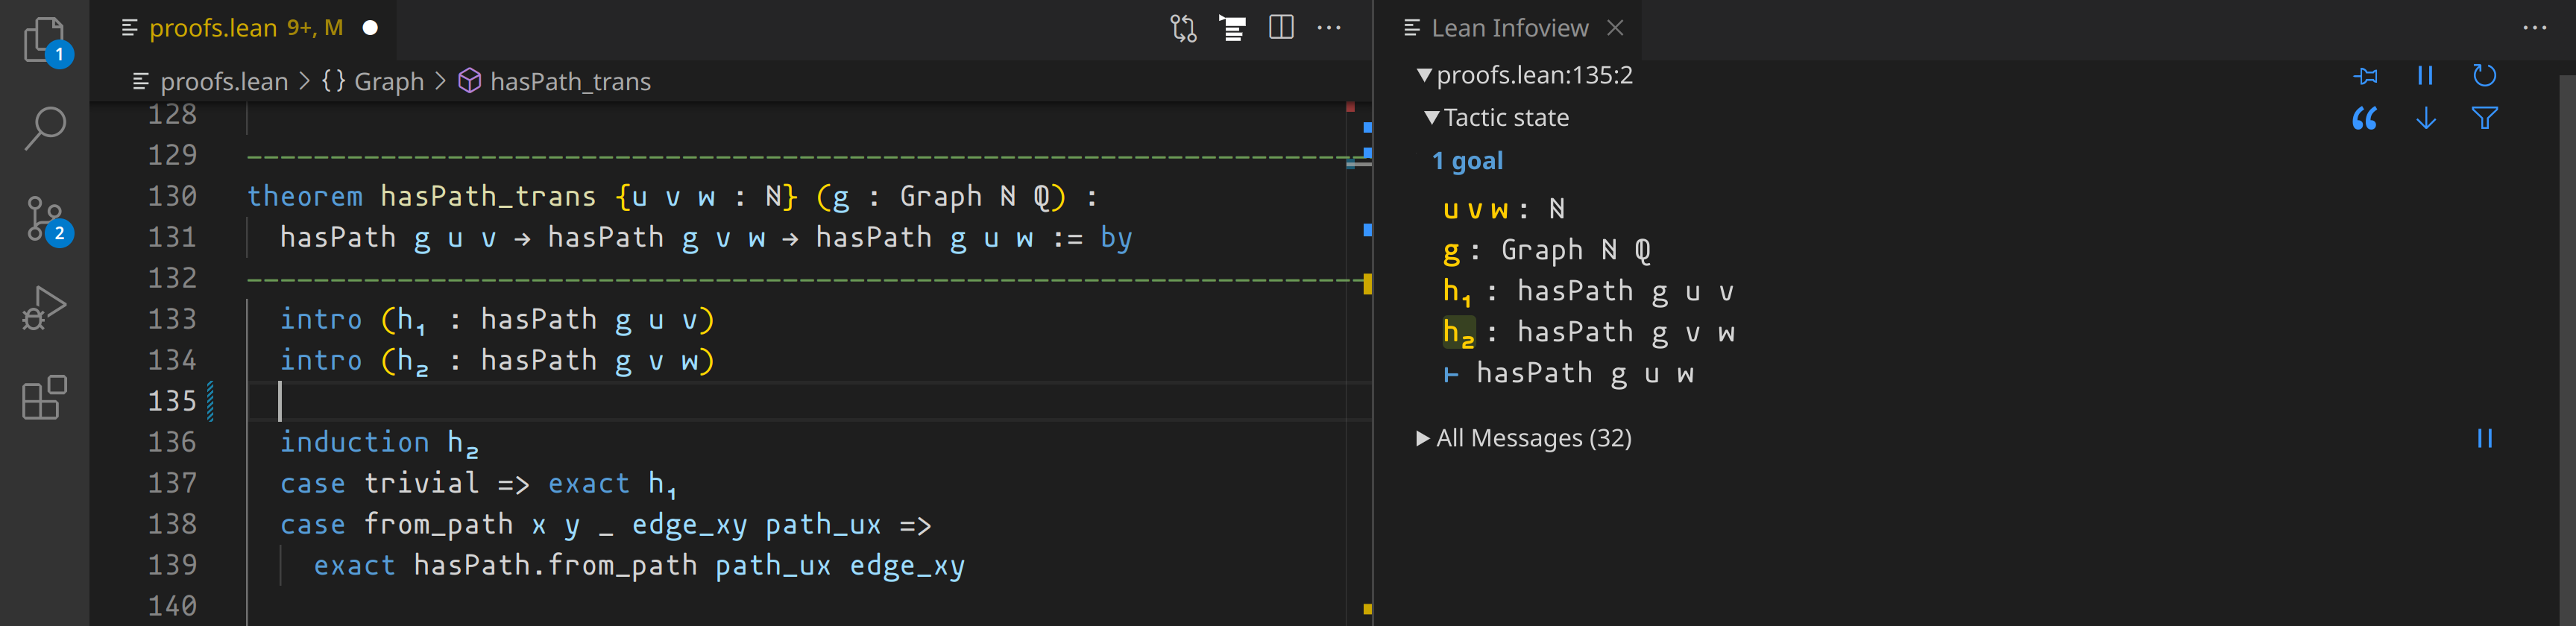
\includegraphics[scale=0.20]{lean4-example.png}
    
    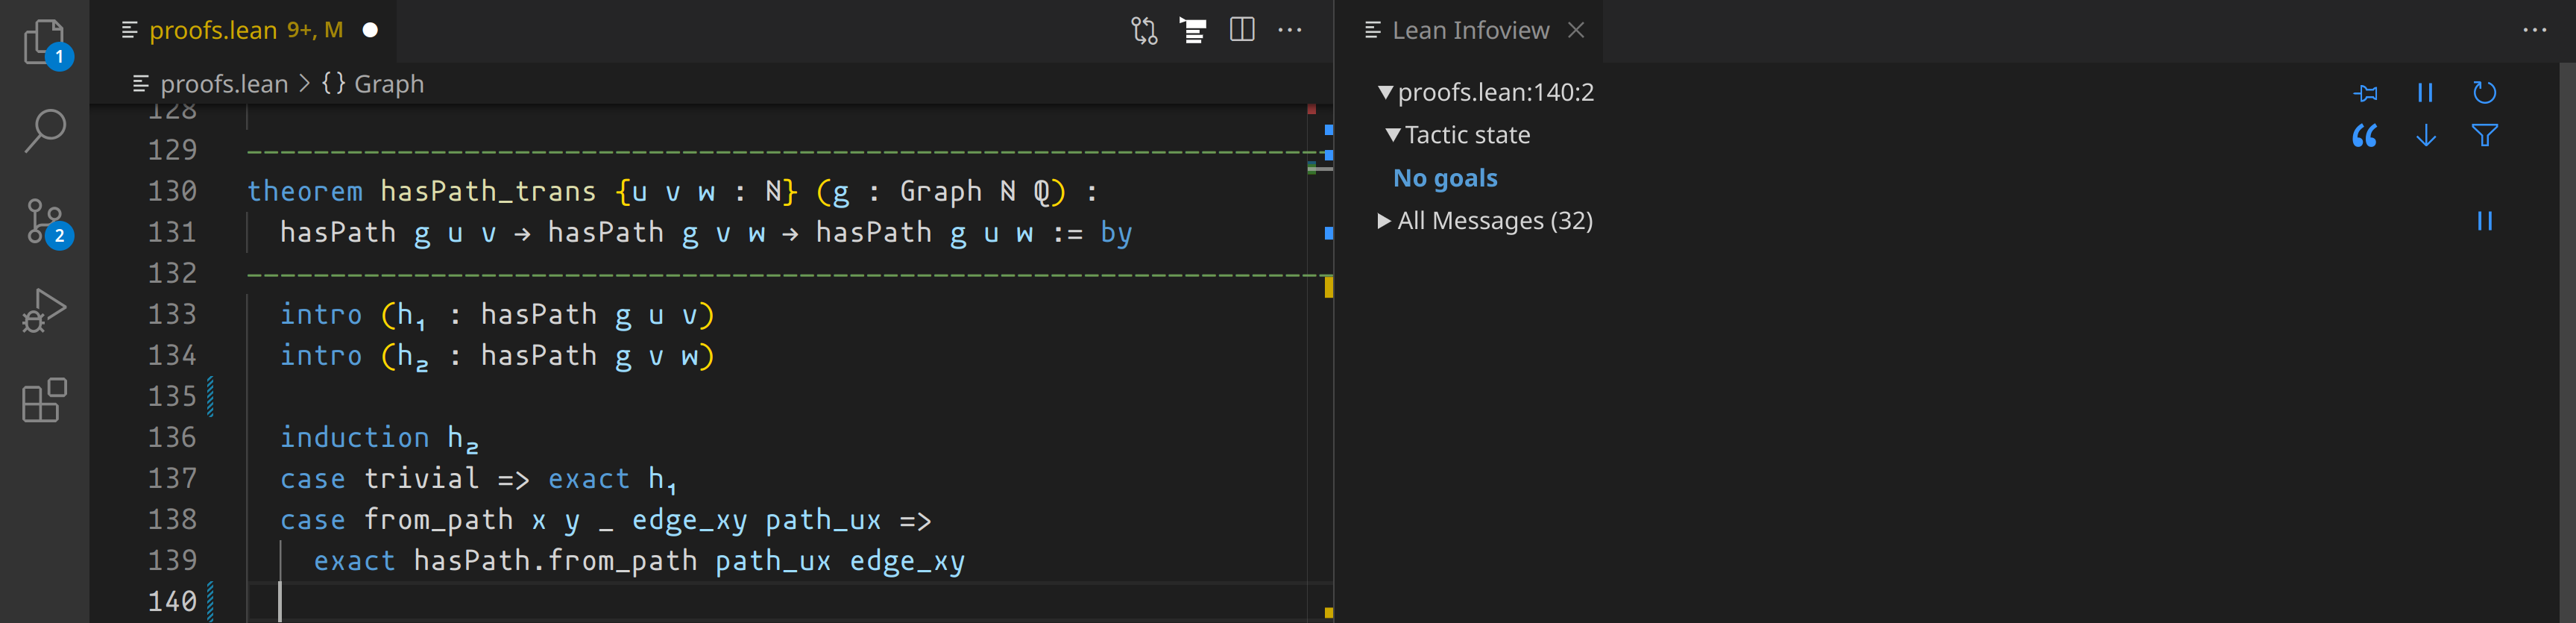
\includegraphics[scale=0.20]{lean4-example2.png}
    \caption{The Lean Infoview (right), at two different lines in the proof.}
    \label{fig:example-code}
\end{figure*}

The Lean Infoview may also show the current context of a proof.  Figure~\ref{fig:example-code} (on the next page) shows an example of this.  The proof on the left shows by induction that if there is a path from $u$ to $v$ in a graph, and a path from $v$ to $w$, then there is a path from $u$ to $w$.  If we place our cursor on line 135, then on the right we see the context of the proof at line 135.  This shows all variables \texttt{u}, \texttt{v}, \texttt{w}, \texttt{g} defined in scope, as well as any assumptions we've made so far \texttt{$h_1$}, \texttt{$h_2$}.  Finally, \texttt{$\vdash$ hasPath g u w} indicates that our goal at this point is to prove that there is a path from \texttt{u} to \texttt{w}.

If we move our cursor to line 140 (the end of this proof), the Lean Infoview tells us that there are no goals left.  This means that the proof is done and formally checked!  Note that proofs that \emph{are not} finished are easily spotted --- the keyword \textcolor{red}{\textbf{\texttt{sorry}}} indicates a goal with no proof.  (We intend to fill in all \textcolor{red}{\textbf{\texttt{sorry}}}'s by the AAAI-24 author feedback window.)


\section{Reproducibility Checklist}

Most of our answers to the Reproducibility Checklist are straightforward (our contribution is theoretical; we state assumptions and claims formally; we provide proofs and intuitions; we cite other theoretical tools we use).  But we we also answered `yes' to some of the experimental questions as well, namely
\begin{itemize}
    \item[10.] \textit{All experimental code used to eliminate or disprove claims is included.} % (yes)
    \item[18.] \textit{All source code required for conducting and analyzing the experiments is included in a code appendix.} % (yes)
    \item[19.] \textit{All source code required for conducting and analyzing the experiments will be made publicly available upon publication of the paper with a license that allows free usage for research purposes.} % (yes)
    \item[20.] \textit{All source code implementing new methods have comments detailing the implementation, with references to the paper where each step comes from.} % (yes)
    \item[22.] \textit{This paper specifies the computing infrastructure used for running experiments (hardware and software), including GPU/CPU models; amount of memory; operating system; names, and versions of relevant software libraries and frameworks.} % (yes)
\end{itemize}
This is because our Lean 4 code doubles as ``experimental code used to eliminate or disprove claims.''  Although we didn't build any counter-models explicitly, Lean's type-checking and resolution system helped us eliminate possible (false) claims in the process of writing our proofs.  (Lean 4 helped us avoid many false starts with Theorem~\ref{reduction_theorem}.)  And when Lean tells us that a proof of a claim is good (there are no goals left), this means that there \emph{aren't} any counter-models for that claim.

We have included all source code in an appendix, and intend to release it under the MIT license.  We have included comments in the source code, with each claim referencing the corresponding claim in the paper.  And in the previous section (as well as in a README.md file), we detail the system requirements for running this code.

There are two questions that we answered `no' to:

\begin{itemize}
    \item[9.] \textit{All theoretical claims are demonstrated empirically to hold.} % NO
    \item[26.] \textit{The significance of any improvement or decrease in performance is judged using appropriate statistical tests (e.g., Wilcoxon signed-rank).} % No
\end{itemize}

For (9), we unfortunately ran out of time to give an effective example or write code testing our reduction on neural networks out in the wild.  Question (26) is not applicable, but at the time of submission the Microsoft CMT system didn't have an option for `not applicable.'

\bibliography{neurosymbolic}
\end{document}